\documentclass[a4paper,UTF8]{ctexart}

\usepackage{amsmath, amsthm, amssymb, amsfonts, hyperref, mathrsfs}%美国数学学会的包+?
\usepackage{geometry} %控制界面
\usepackage{bookmark}
\usepackage{fancyhdr} % header & footer
\usepackage{appendix} % 附录
\usepackage{tikz} %作图
\usepackage{graphicx} %插入图片的宏包
\usepackage{float} %设置图片浮动位置的宏包
%\usepackage{subfigure} %插入多图时用子图显示的宏包
\usepackage{listings} %引用代码
\usepackage{physics,mathtools} %物理数学工具
\usepackage{comment}
\usepackage{framed}
\usepackage{caption}
\usepackage{subcaption}
\geometry{top=2.5cm,bottom=2.5cm,left=2.5cm,right=2.5cm} % 布局要求
\pagestyle{fancy} % fancy分格
\fancyhf{} % 清除所有页眉页脚
\renewcommand\headrulewidth{0.6pt}
\renewcommand\footrulewidth{0.6pt}
% font
\setCJKmainfont{Noto Serif CJK SC}[BoldFont={Noto Serif CJK SC Bold}, ItalicFont=]
\lhead{何金铭 PB21020660$\mid$座位号:4}
\chead{双光子HOM干涉实验报告}
\rhead{\thepage}
\lfoot{2024.4.9}
\rfoot{USTC}
%\bibliographystyle{plain} % 引用样式
\everymath{\displaystyle} % display
%============================================================

\begin{document}

\begin{center}
    \textbf{\Large 双光子HOM干涉实验报告}
    \par \text{\large 何金铭 PB21020660}
\end{center}

实验目的,实验原理,实验内容已于预习报告中给出,本实验报告中不再复述。

\section{实验结果与分析}

\subsection{光子单路计数和复合计数与泵浦功率的关系实验}

\begin{table}[H]
    \centering
    \caption{单路计数和符合计数与泵浦功率的关系表}
    \begin{tabular}{|l|l|l|l|}
    \hline
        光强 mW & 单路计数 Counts & 单路计数 Counts & 符合计数 Counts \\ \hline
        0.03 & 19000 & 15000 & 878 \\ \hline
        0.1 & 37000 & 35000 & 2777 \\ \hline
        0.2 & 66000 & 66000 & 10521 \\ \hline
        0.4 & 128000 & 123000 & 22290 \\ \hline
    \end{tabular}
\end{table}

\begin{figure}[H]
    \centering
    \begin{minipage}[b]{0.9\textwidth}
        \centering
        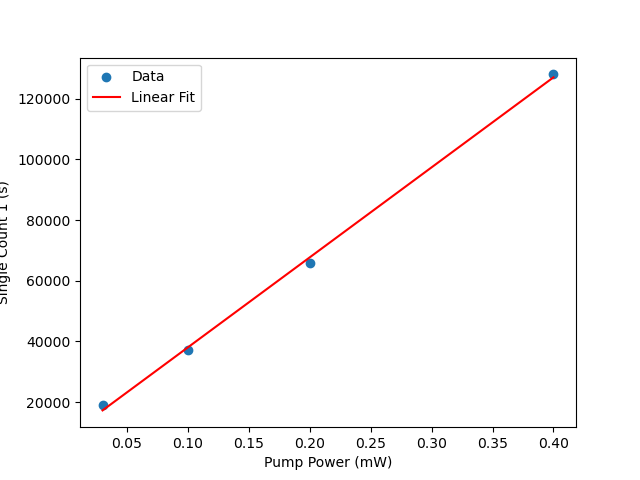
\includegraphics[width=0.9\textwidth]{./ffig1.png}
        \caption{光强-单路1计数图}
    \end{minipage}
\end{figure}

\begin{figure}[H]
    \centering
    \begin{minipage}[b]{0.9\textwidth}
        \centering
        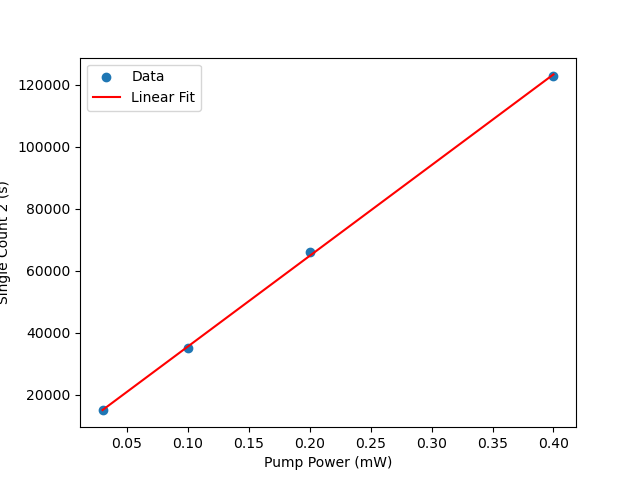
\includegraphics[width=0.9\textwidth]{./ffig2.png}
        \caption{光强-单路2计数图}
    \end{minipage}
\end{figure}

\begin{figure}[H]
    \centering
    \begin{minipage}[b]{0.9\textwidth}
        \centering
        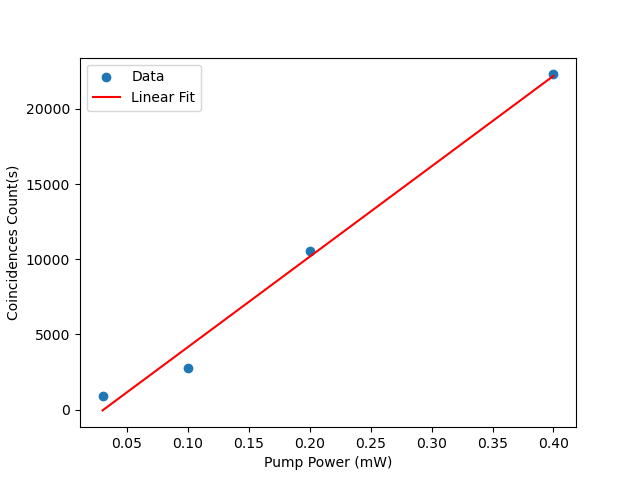
\includegraphics[width=0.9\textwidth]{./ffig3.png}
        \caption{光强-符合计数图}
    \end{minipage}
\end{figure}

如上图所示,单路计数和符合计数都正比于泵浦光子数即泵浦功率,符合预习报告中的公式(5)、(6),合理。

\subsection{符合信噪比与泵浦功率的关系}

\begin{table}[H]
    \centering
    \caption{符合信噪比与泵浦功率的关系表}
    \begin{tabular}{|l|l|l|l|}
    \hline
        光强 mW & 符合计数 Counts & 暗符合计数 Counts & CAR \\ \hline
        0.03 & 878 & 4 & 220.5 \\ \hline
        0.1 & 2777 & 7 & 397.71429 \\ \hline
        0.2 & 10521 & 18 & 585.5 \\ \hline
        0.4 & 22290 & 50 & 446.8 \\ \hline
        0.6 & 35957 & 98 & 367.90816 \\ \hline
        1 & 54213 & 210 & 259.15714 \\ \hline
        1.5 & 85590 & 520 & 165.59615 \\ \hline
        2 & 10935 & 780 & 15.01923 \\ \hline
        2.5 & 130835 & 1000 & 131.835 \\ \hline
        3.06 & 149005 & 1500 & 100.33667 \\ \hline
        4.02 & 173334 & 2000 & 87.667 \\ \hline
    \end{tabular}
\end{table}

用预习报告中的公式(7)拟合得:

\begin{figure}[H]
    \centering
    \begin{minipage}[b]{0.9\textwidth}
        \centering
        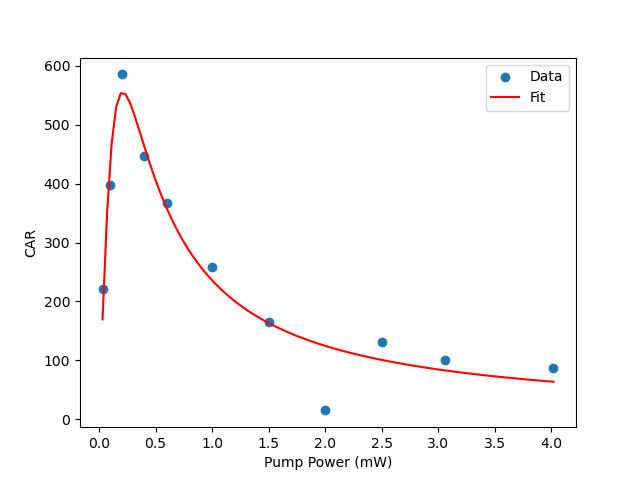
\includegraphics[width=0.9\textwidth]{./ffig4.png}
        \caption{光强-CAR图}
    \end{minipage}
\end{figure}

发现随着功率的增加,CAR值先增加后减小,在增加的区间主要是光子产生率增加,相对于暗噪声的有效符合数增加,然而在高产生率情况下,由于多光子效应明显,导致符合信噪比下降。

\subsection{HOM干涉曲线测量}

\begin{table}[H]
    \centering
    \caption{HOM 干涉曲线记录表}
    \begin{tabular}{|l|l|l|l|}
    \hline
        位置 mm & 符合计数 Counts & 位置 mm & 符合计数 Counts \\ \hline
        16 & 84224 & 16.83 & 40319 \\ \hline
        16.1 & 85275 & 16.84 & 41520 \\ \hline
        16.2 & 84477 & 16.85 & 39465 \\ \hline
        16.3 & 84635 & 16.86 & 41783 \\ \hline
        16.4 & 84073 & 16.87 & 38952 \\ \hline
        16.5 & 82151 & 16.88 & 41577 \\ \hline
        16.6 & 79213 & 16.89 & 42050 \\ \hline
        16.7 & 52606 & 16.9 & 42020 \\ \hline
        16.75 & 45010 & 16.95 & 51766 \\ \hline
        16.76 & 44086 & 17 & 70114 \\ \hline
        16.77 & 42755 & 17.1 & 72595 \\ \hline
        16.78 & 43079 & 17.2 & 72407 \\ \hline
        16.79 & 42574 & 17.3 & 74381 \\ \hline
        16.8 & 40937 & 17.4 & 70928 \\ \hline
        16.81 & 41096 & 17.5 & 67575 \\ \hline
        16.82 & 41343 & & \\ \hline
    \end{tabular}
\end{table}

用预习报告中的公式(2)拟合得:

\begin{figure}[H]
    \centering
    \begin{minipage}[b]{0.9\textwidth}
        \centering
        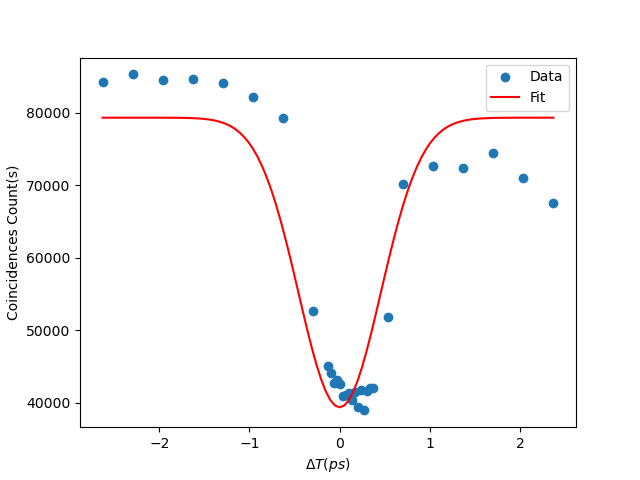
\includegraphics[width=0.9\textwidth]{./ffig6.png}
        \caption{HOM干涉曲线,符合计数与光子相对延迟时间的关系}
    \end{minipage}
\end{figure}

发现存在一定的误差

\section{实验总结}

\begin{enumerate}
    \item 发现单路计数和符合计数都正比于泵浦光子数即泵浦功率
    \item 发现发现随着功率的增加,CAR值先增加后减小,在增加的区间主要是光子产生率增加,相对于暗噪声的有效符合数增加,然而在高产生率情况下,由于多光子效应明显,导致符合信噪比下降。
    \item 实验测得了HOM干涉曲线,发现存在一定的误差,可能是:
    \begin{enumerate}
        \item 曲线左右高低不一致是因为两路单路符合计数有一些差异,这是由于左右单路空间-光纤耦合效率不同以及其他种种因素造成的。
        \item 曲线底部数据不平滑,可能是由于实验中的环境噪声等因素导致的。
    \end{enumerate}
\end{enumerate}

\section{思考题}

\subsection{观测HOM干涉需要满足哪些条件?}

\begin{enumerate}
    \item 双光子源:HOM干涉是基于双光子的相互作用效应,因此需要使用双光子源来产生两个光子的纠缠态或准纠缠态。
    \item 空间和时间匹配:两个入射光子应该在空间和时间上足够接近,以便在光学器件中相互干涉。这意味着它们的空间模式(波前形状)和时间延迟应该足够匹配
    \item 50:50分束器:HOM干涉通常使用一个50:50的光学分束器(如非极化的光学器件或偏振分束器)来将两个光子分别引导到两个不同的路径上。分束器应具有高的耦合效率和低的损耗,以保持干涉的高可见度
    \item 光子计数:观测HOM干涉需要对来自两个输出路径的光子进行单光子探测和计数。这样可以测量干涉效应,并计算出干涉可见度和干涉图案。
    \item 相干性:观测HOM干涉需要光子源具有足够的相干性,以产生干涉图案。相干性可以通过光子源的频谱特性和相干长度来衡量。
    \item 背景噪声和误差控制:在HOM干涉实验中,需要控制背景噪声和误差,以获得清晰的干涉信号。这包括控制环境的光和振动噪声,并采取适当的探测器和测量技术来减少噪声和误差的影响。
\end{enumerate}

\subsection{自发参量下转换过程中,光子的产生率依赖于哪些参数?其辐射带宽与什么有关?}

光子的产生率依赖于以下参数:

\begin{enumerate}
    \item 光子源的非线性系数:SPDC是一种非线性过程,光子的产生率与材料或器件的非线性系数有关。常见的非线性材料包括二硫化铟(InSb)、铁电晶体和周期极化波导等。
    \item 抽运光子的功率:SPDC过程通常是通过抽运光子与非线性材料的相互作用来实现的。抽运光子的功率越高,产生的信号光子和辅助光子的产生率也就越高。
    \item 抽运光子的波长:抽运光子的波长决定了SPDC过程中产生的信号光子和辅助光子的波长。SPDC过程是一个能量守恒的过程,信号光子和辅助光子的波长满足能量守恒条件。
    \item 非线性材料的长度:非线性材料的长度决定了光子在其中的作用时间和相互作用的强度。较长的非线性材料长度可以增加光子的产生率,但也会引入相位匹配条件的挑战。
\end{enumerate}

辐射带宽的大小与非线性材料的色散特性、非线性过程的相位匹配条件和非线性材料的长度等因素有关。

\subsection{符合与暗符合信噪比与哪些因素有关?}

\begin{enumerate}
    \item 信号强度:符合事件的信号强度是CAR的一个重要影响因素。较高的信号强度可以提高符合事件的计数率,从而增加CAR。在光学实验中,信号强度通常与光子的产生率、探测器的灵敏度以及光学器件的传输效率等因素相关。
    \item 底座噪声:底座噪声是指在没有信号的情况下探测器产生的暗计数。底座噪声的大小取决于探测器的特性、环境噪声以及测量系统的设计和优化等因素。较低的底座噪声可以提高CAR,因为它减少了暗符合事件的计数率。
    \item 暗计数率:暗计数率是指在没有信号输入时,探测器产生的计数率。暗计数率可以由探测器的特性和环境条件引起,例如热噪声、光电子倍增管的暗电子产生率等。较低的暗计数率可以提高CAR,因为它减少了暗符合事件的计数率。
    \item 测量时间:测量时间对CAR的影响非常明显。较长的测量时间可以积累更多的符合事件和暗符合事件的计数,从而提高CAR。然而,长时间的测量也可能增加底座噪声和暗计数率的影响。
\end{enumerate}

\subsection{如何通过HOM干涉来表征光子的辐射带宽?如何通过HOM干涉测量一个已知折射率的透明材料的厚度?}

通过HOM干涉来表征光子的辐射带宽的方法如下:

已知符合计数表达式为:

\begin{equation}
    N_{cd} = \kappa (T^2+R^2)[1-\frac{2RT}{T^2+R^2}\exp{(-\Delta \omega \delta \tau)}]
\end{equation}

可以通过采的数据和上述公式拟合得到$\Delta \omega$,即为光子的辐射带宽。

通过HOM干涉测量已知折射率的透明材料的厚度,具体方法如下:

在HOM干涉的输入光路(迈克尔逊干涉仪的一路)中加入样品,加入之后测得的HOM干涉曲线干涉峰的X轴位置,即迈克尔逊干涉仪一路反射镜的位置,可以推测出加入样品前后的光程差,而又已知折射率,即可求得厚度。

\end{document}